\chapter{Final Evaluation}
\label{chap:evaluation}
\centerline{\rule{149mm}{.02in}}
\vspace{2cm}

We have shown that the point $kd$-tree greatly outperforms the Pyramid tree for the two scientific datasets. For all synthetic data and the 3D point cloud dataset, the Pyramid tree is faster, especially with regard to point deletion.

This chapter will explore the reasons for this, determining what characteristics the astrophysics dataset cause the performance of the structures to degenerate. The chapter will conclude by discussing the types of data suitable for the Pyramid Tree and $kd$-Tree, along with some further discussion on the implications of the results from this evaluation.

\section{Characteristics of Astrophysics Dataset}
\label{sec:data-characteristics}

A dataset is considered \textit{skewed} if a greater number of points are present in certain regions of the data space than other regions of the space. That is, the underlying frequency or probability distribution of point locations is non-uniform. Figure \ref{fig:frequency-distributions} visualises uniform, Gaussian and skewed frequency distributions using histograms. Intuitively, the skewness of a dataset increases as the difference between the frequency of points in different spatial regions increases.

\begin{figure}
	\begin{center}
		\begin{subfloat}[Uniform\label{fig:uniform-freq-distribution}]{%
			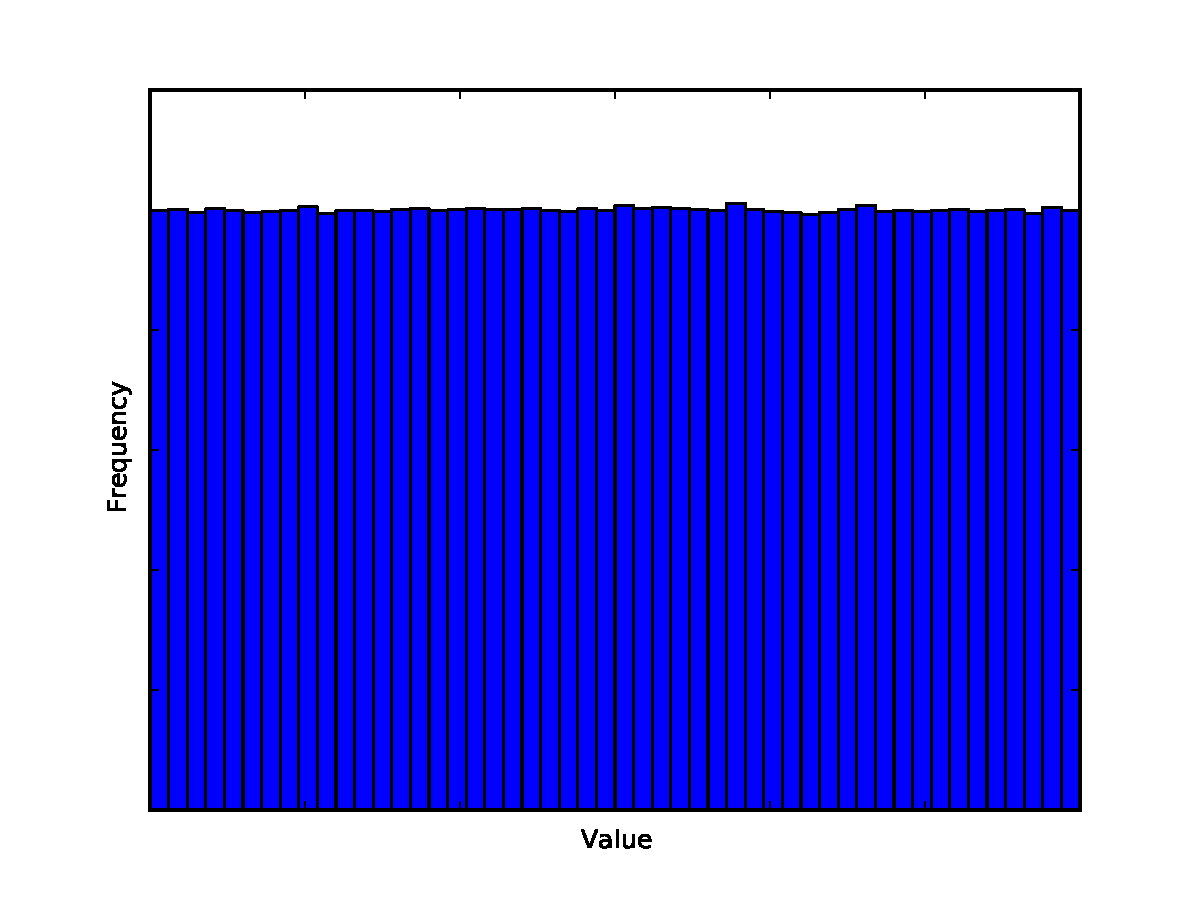
\includegraphics[scale=0.25]{figures/freqdist_uniform.pdf}
		}
		\end{subfloat}~
		\begin{subfloat}[Gaussian\label{fig:gaussian-freq-distribution}]{%
			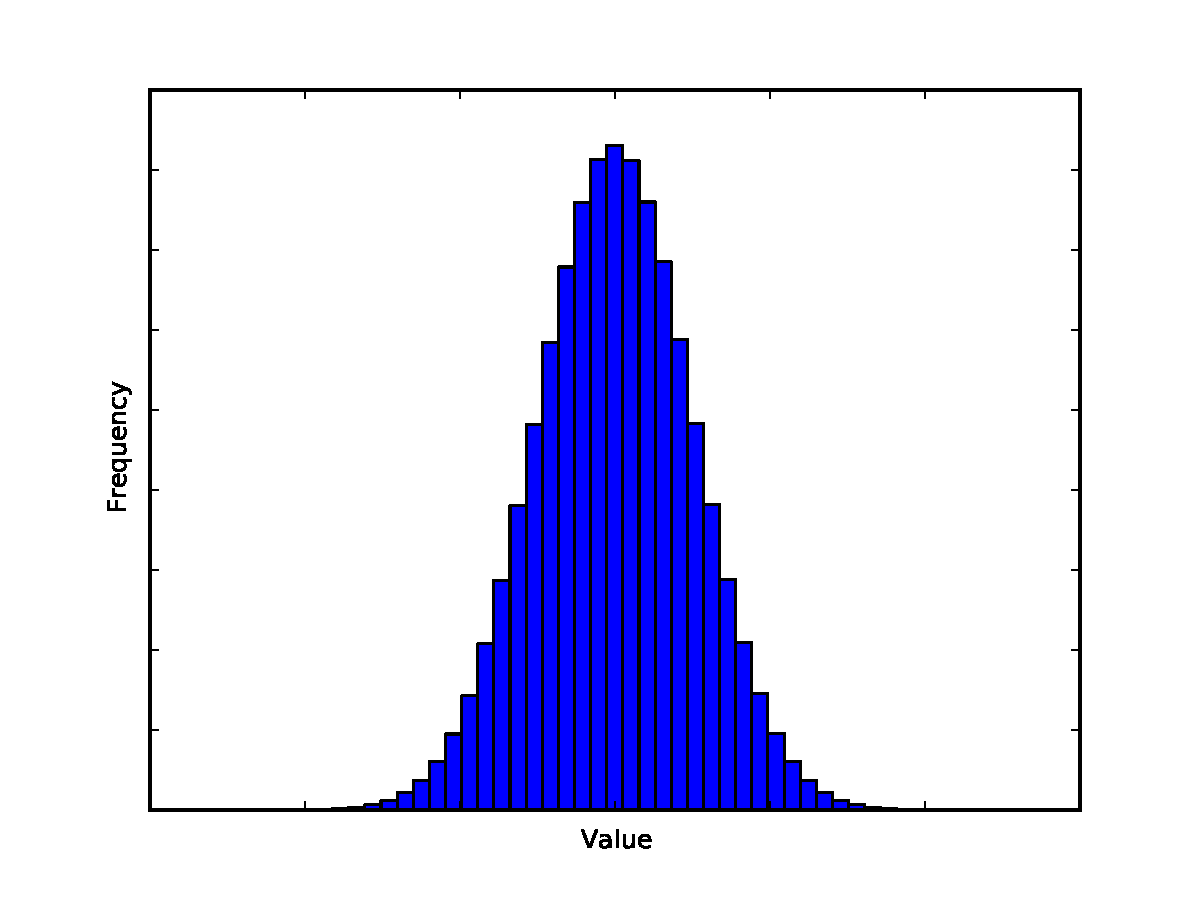
\includegraphics[scale=0.25]{figures/freqdist_gaussian.pdf}
		}
		\end{subfloat}~
		\begin{subfloat}[Gamma (Skewed)\label{fig:skewed-freq-distribution}] {%
			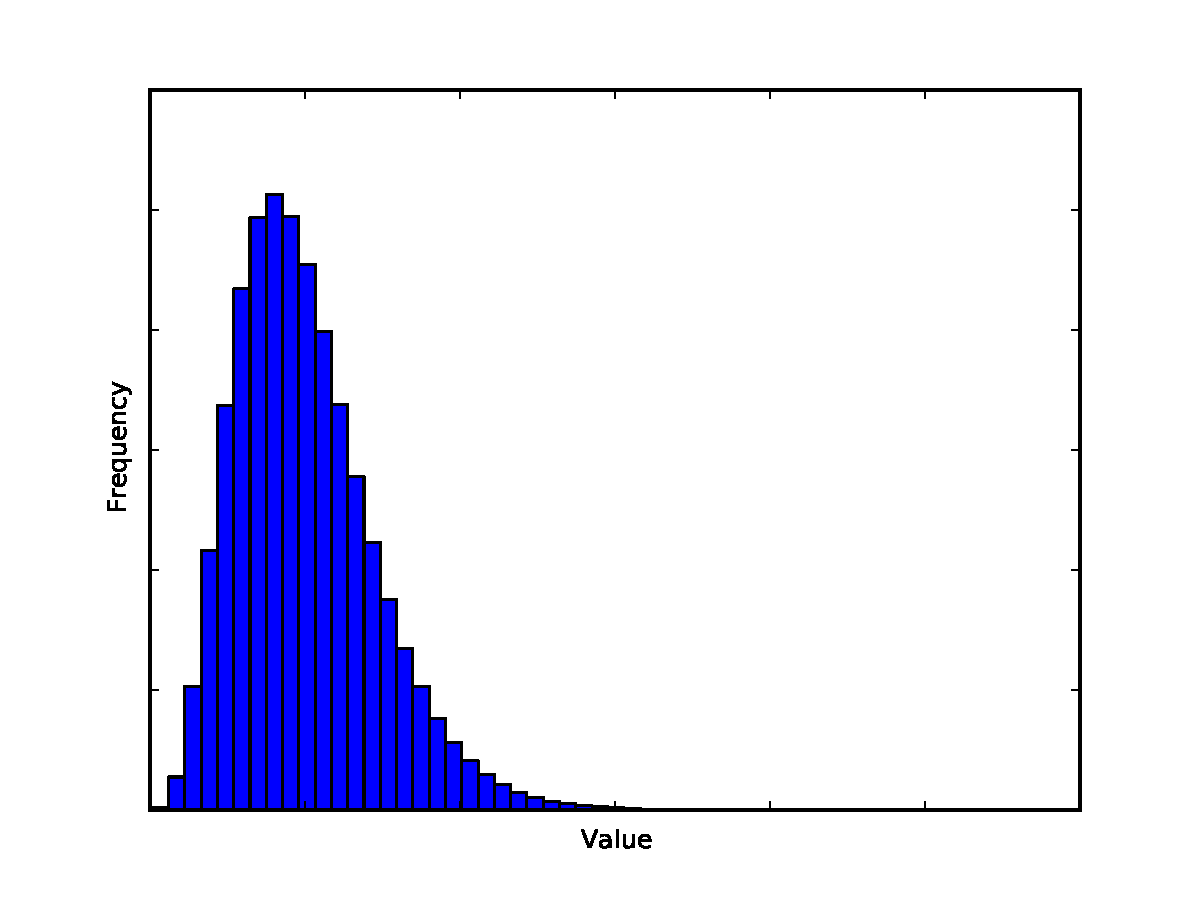
\includegraphics[scale=0.25]{figures/freqdist_gamma.pdf}
		}
		\end{subfloat}
	\end{center}

	\caption{Three Types of Frequency Distributions}
	\label{fig:frequency-distributions}
\end{figure}

Histograms are used to visualise the frequency distributions of one-dimensional data. Since this project deals with multi-dimensional data, multiple histograms, one for each dimension, will be produced. The astrophysics dataset was computed using a 3D sampling lattice, computing ten fields at each point. The original simulation imposes continuous, spatial relationships between the points through interpolation \cite{TODO}. TODO Carr et. al \cite{histograms-and-isosurfaces}.

While Carr et. al have shown that   TODO: justify why histograms will be used and their limitations

Ten histograms have been generated using each dimension of the astrophysics dataset. Figure \ref{fig:astrophysics-histograms} shows the histograms of dimensions 1, 2, 3 and 7. The histograms for the remaining dimensions are provided in Appendix \ref{sec:app-histograms}, and not here, because they have distributions similar to the dimensions shown here.

\begin{figure}
	\begin{center}
		\begin{subfloat}[Dimension 1 (total particle density)]{%
			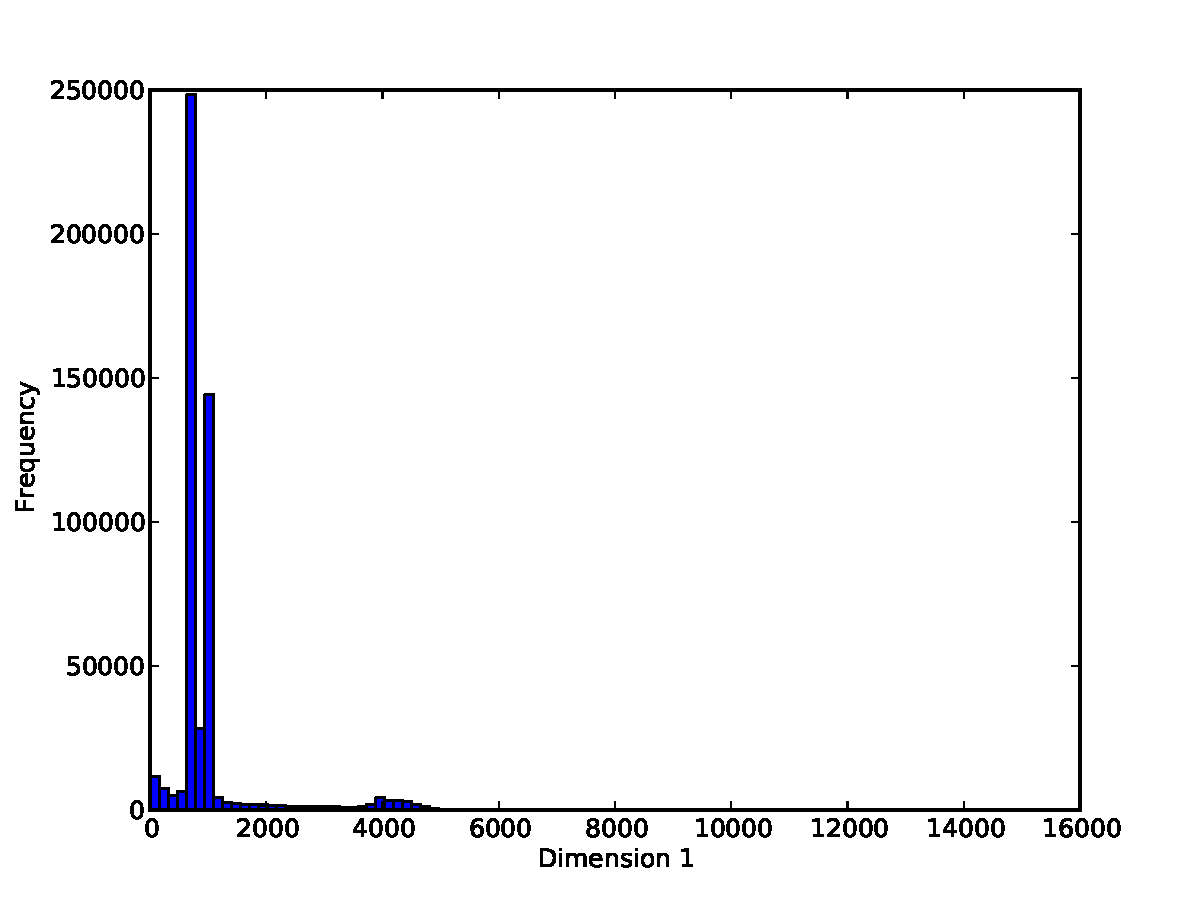
\includegraphics[scale=0.36]{figures/histograms/astrophysics_500000_0.pdf}
		}
		\end{subfloat}~
		\begin{subfloat}[Dimension 2 (gas temperature)]{%
			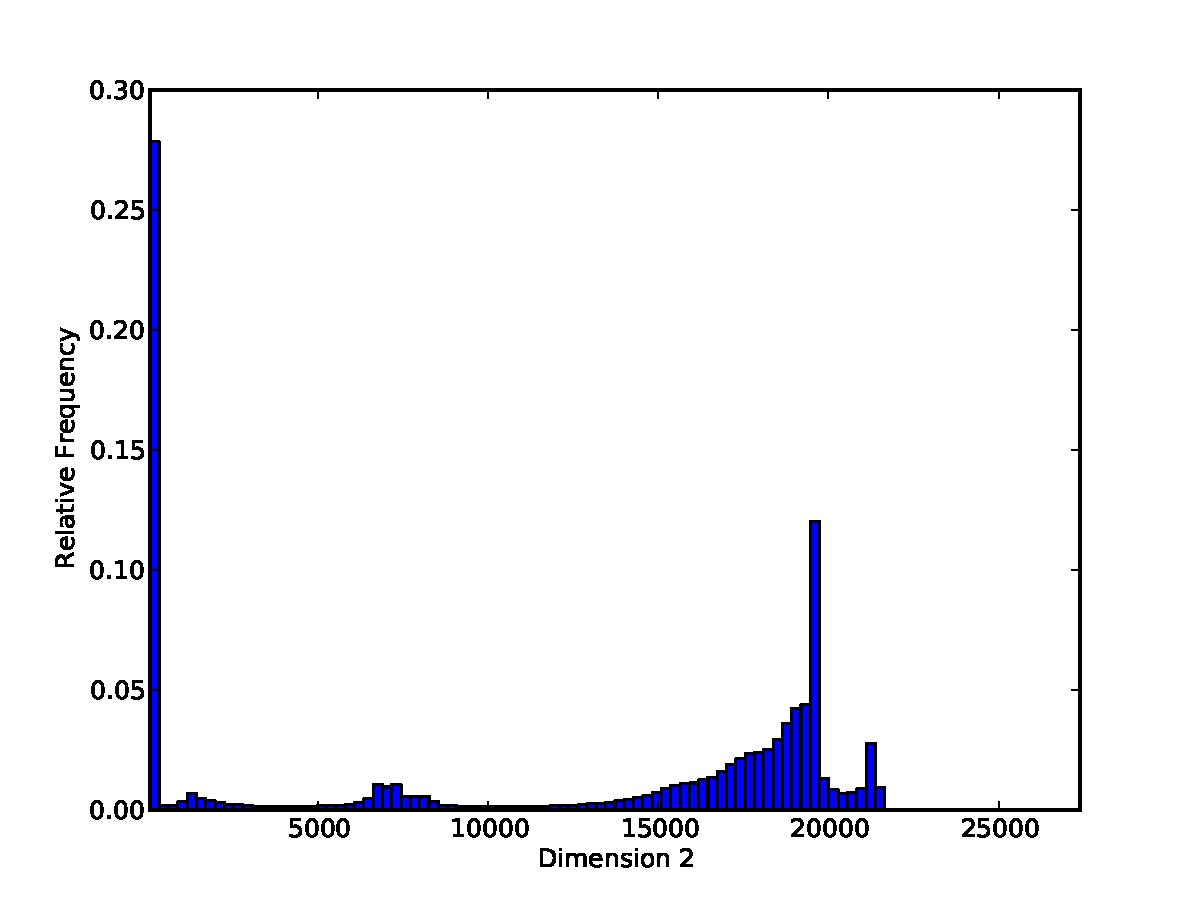
\includegraphics[scale=0.36]{figures/histograms/astrophysics_500000_1.pdf}
		}
		\end{subfloat}
	\end{center}

	\caption{Frequency Distributions of Dimensions 1 and 2 of Astrophysics Dataset}
	\label{fig:astrophysics-histograms1}
\end{figure}

\begin{figure}
	\begin{center}
		\begin{subfloat}[Dimension 3 (H mass abundance)]{%
			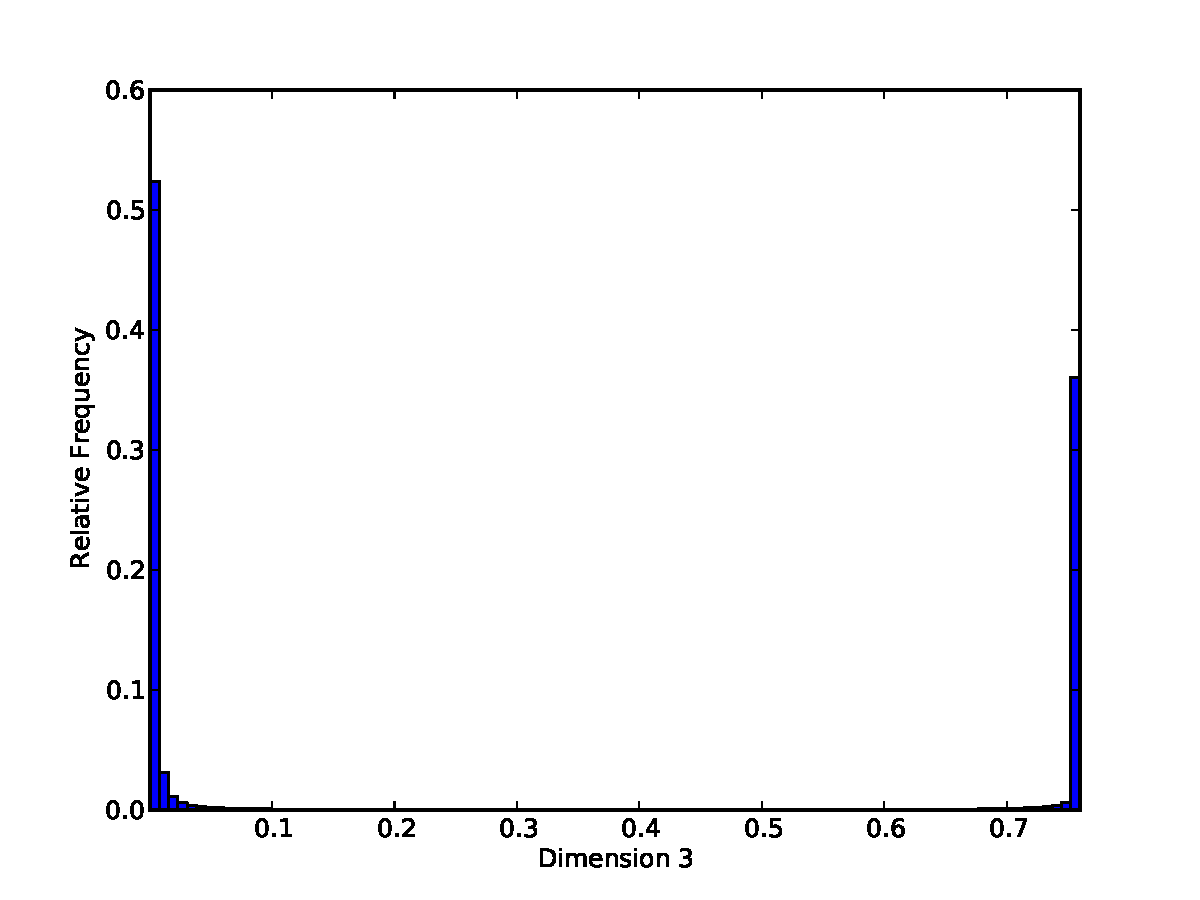
\includegraphics[scale=0.36]{figures/histograms/astrophysics_500000_2.pdf}
		}
		\end{subfloat}~
		\begin{subfloat}[Dimension 7 (He${}^{++}$ mass abundance)]{%
			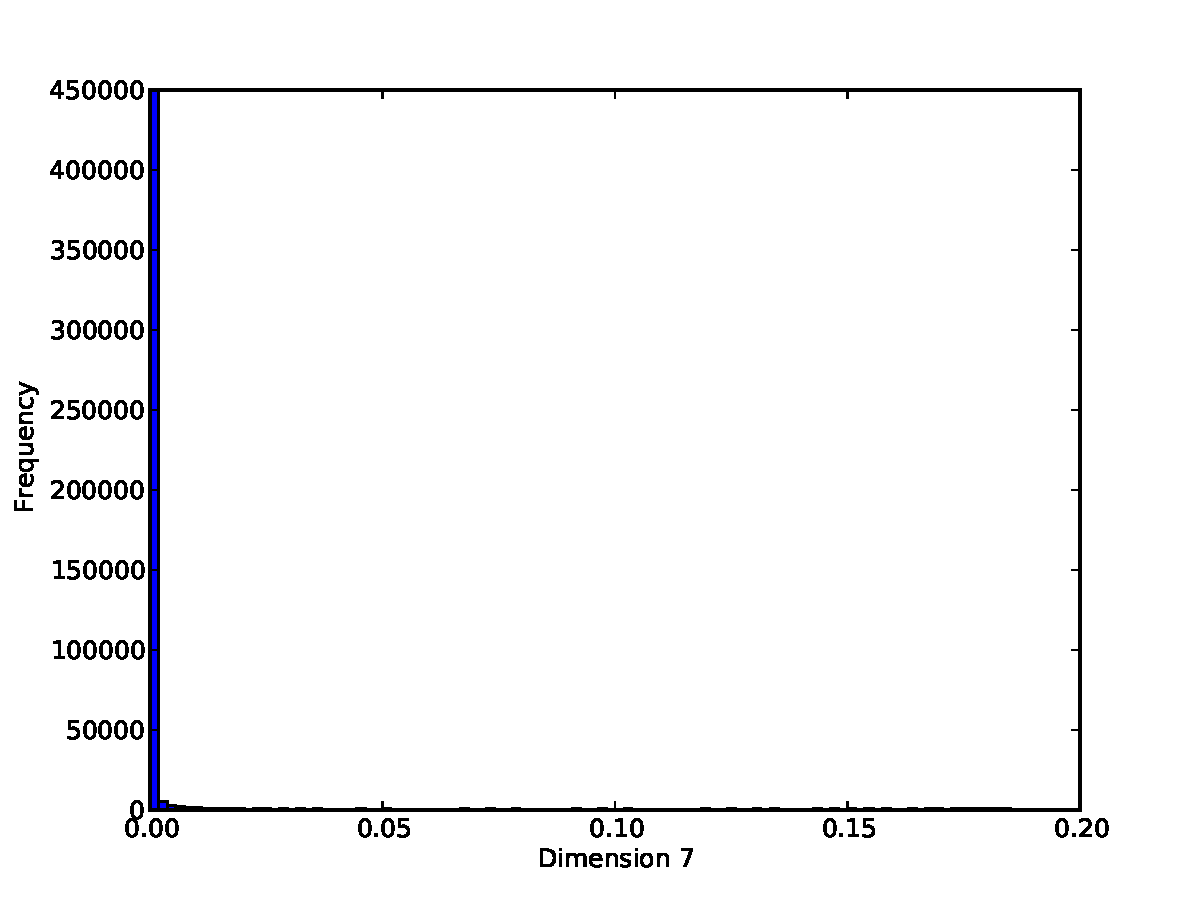
\includegraphics[scale=0.36]{figures/histograms/astrophysics_500000_6.pdf}
		}
		\end{subfloat}
	\end{center}

	\caption{Frequency Distributions of Dimensions 3 and 7 of Astrophysics Dataset}
	\label{fig:astrophysics-histograms2}
\end{figure}

Total particle density (D) and gas temperature (G), the first two dimensions, appear to have the greatest

TODO: REMARKS on histograms and what it means

\section{Effect of Distribution on Pyramid Tree}

TODO

\section{Effect of Distribution on $kd$-Tree}

TODO

\section{Why So Sparse?}

TODO: conjecture on why the astrophysics dataset is so sparse -- referencing literature and how this might support stuff

\section{Suitable Data for Index Structures}

TODO

\section{Project Process}

TODO